\chapter{Evaluierung}
\label{chap:eval}
\todo[size=\small, color=blue!40, inline]{Kapitel: Evaluierung}%
\begin{itemize}
 \item wie skaliert das System / bringt es was?
 \item Cache löschen - neu laden -> Zeit messen
 \item Verschiedene Kamerapositionen:
 \begin{itemize}
  \item Turbine
  \item Cockpit
  \item Heck
  \item ``Businessclass''
  \item seitlich von Außen
 \end{itemize}
 \item Erklärung der Tests \& Diagramme
 \item Balancierung durch c-Collision Protokoll / die Varianz
\end{itemize}
\todo[size=\small, inline]{Grafiken mit echten Daten füllen!}%




\begin{figure}
\centering
%%%%%%%%%%%%%%%%%%%%%%%%%%%%%%%%%%%%%%%%%%%%%%%%%%%%%%%%%
% Beispieldiagramm mit pgfplot und datenfile
%%%%%%%%%%%%%%%%%%%%%%%%%%%%%%%%%%%%%%%%%%%%%%%%%%%%%%%%%

\begin{tikzpicture}
  \begin{axis}[xlabel=Kameraposition, ylabel={Zeit (in Sekunden)}]
    \addplot table[col sep=comma,x index=0,y index=1,header=false] {data/ReloadTest_R2_D2.2010-1-24.log};
    \addlegendentry{DataNode0}
    \addplot table[col sep=comma,x index=0,y index=2,header=false] {data/ReloadTest_R2_D2.2010-1-24.log};
    \addlegendentry{DataNode1}
  \end{axis}
\end{tikzpicture}

  \caption{Ein Beispieldiagramm mit Datenfile.}
  \label{fig:eval:diag1}
\end{figure}

\begin{figure}
\centering
%%%%%%%%%%%%%%%%%%%%%%%%%%%%%%%%%%%%%%%%%%%%%%%%%%%%%%%%%
% Testdiagramm 2
%%%%%%%%%%%%%%%%%%%%%%%%%%%%%%%%%%%%%%%%%%%%%%%%%%%%%%%%%


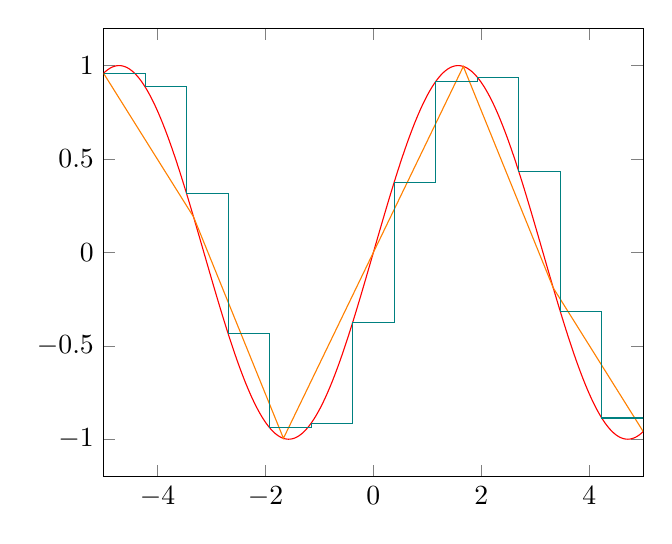
\begin{tikzpicture}
  \begin{axis}[enlarge x limits=false]
    \addplot[red,samples=500] {sin(deg(x))};
    \addplot[orange,samples=7] {sin(deg(x))};
    \addplot[teal,const plot,samples=14] {sin(deg(x))};
  \end{axis}
\end{tikzpicture}

  \caption{Beispieldiagramm 2.}
  \label{fig:eval:diag2}
\end{figure}

\begin{figure}
\centering
%%%%%%%%%%%%%%%%%%%%%%%%%%%%%%%%%%%%%%%%%%%%%%%%%%%%%%%%%
% Testdiagramm 3
%%%%%%%%%%%%%%%%%%%%%%%%%%%%%%%%%%%%%%%%%%%%%%%%%%%%%%%%%


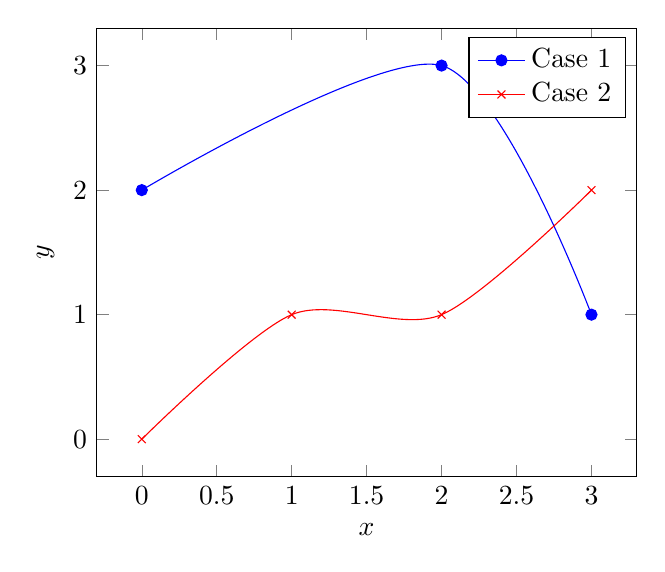
\begin{tikzpicture}
  \begin{axis}[xlabel=$x$, ylabel=$y$]
    \addplot[smooth,mark=*,blue] plot coordinates {
      (0,2)
      (2,3)
      (3,1)
    };
    \addlegendentry{Case 1}
    \addplot[smooth,color=red,mark=x]
        plot coordinates {
            (0,0)
            (1,1)
            (2,1)
            (3,2)
        };
    \addlegendentry{Case 2}
  \end{axis}
\end{tikzpicture}

  \caption{Beispieldiagramm 3.}
  \label{fig:eval:diag3}
\end{figure}

\begin{figure}
\centering
%%%%%%%%%%%%%%%%%%%%%%%%%%%%%%%%%%%%%%%%%%%%%%%%%%%%%%%%%
% Testdiagramm 4
%%%%%%%%%%%%%%%%%%%%%%%%%%%%%%%%%%%%%%%%%%%%%%%%%%%%%%%%%


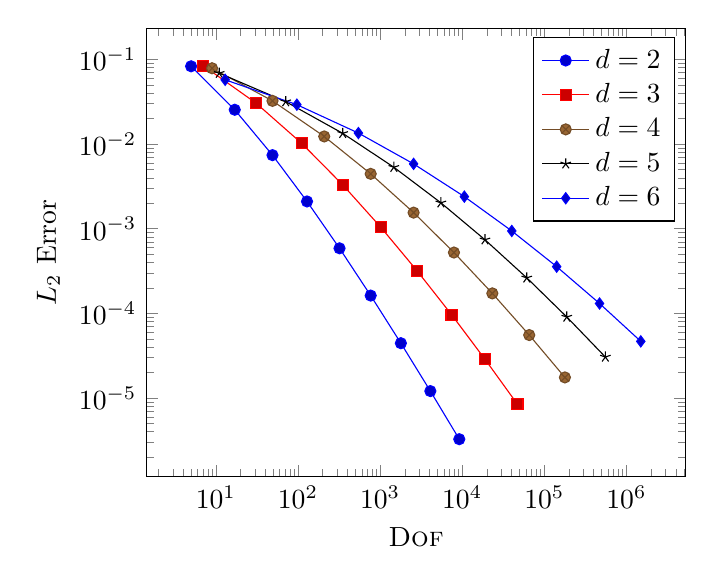
\begin{tikzpicture}
    \begin{loglogaxis}[
        xlabel=\textsc{Dof},
        ylabel=$L_2$ Error
    ]
    \axispath\draw
            (7.49165,-10.02171)
        |-  (8.31801,-11.32467)
        node[near start,left] {$\frac{dy}{dx} = -1.58$};
      \addplot plot coordinates {
        (5,     8.312e-02)
        (17,    2.547e-02)
        (49,    7.407e-03)
        (129,   2.102e-03)
        (321,   5.874e-04)
        (769,   1.623e-04)
        (1793,  4.442e-05)
        (4097,  1.207e-05)
        (9217,  3.261e-06)
    };

    \addplot plot coordinates {
        (7,     8.472e-02)
        (31,    3.044e-02)
        (111,   1.022e-02)
        (351,   3.303e-03)
        (1023,  1.039e-03)
        (2815,  3.196e-04)
        (7423,  9.658e-05)
        (18943, 2.873e-05)
        (47103, 8.437e-06)
    };

    \addplot plot coordinates {
        (9, 7.881e-02)
        (49,    3.243e-02)
        (209,   1.232e-02)
        (769,   4.454e-03)
        (2561,  1.551e-03)
        (7937,  5.236e-04)
        (23297, 1.723e-04)
        (65537, 5.545e-05)
        (178177,    1.751e-05)
    };

    \addplot plot coordinates {
        (11,    6.887e-02)
        (71,    3.177e-02)
        (351,   1.341e-02)
        (1471,  5.334e-03)
        (5503,  2.027e-03)
        (18943, 7.415e-04)
        (61183, 2.628e-04)
        (187903,    9.063e-05)
        (553983,    3.053e-05)
    };

    \addplot plot coordinates {
        (13,    5.755e-02)
        (97,    2.925e-02)
        (545,   1.351e-02)
        (2561,  5.842e-03)
        (10625, 2.397e-03)
        (40193, 9.414e-04)
        (141569,    3.564e-04)
        (471041,    1.308e-04)
        (1496065,   4.670e-05)
    };
    \legend{$d=2$\\$d=3$\\$d=4$\\$d=5$\\$d=6$\\}

    \end{loglogaxis}
\end{tikzpicture}

  \caption{Beispieldiagramm 4.}
  \label{fig:eval:diag4}
\end{figure}

